\chapter{Uvod}

\section{Pravzaprav uvod}
\emph{Matematika} je veda, ki govori o vzorcih, simetrijah, oblikah in lepoti medsebojnega prepletanja vsega tega. Je čudovit abstrakten svet, ki ne dopušča vsakomur, da bi vstopil vanj. Obiskovalci morajo namreč pri vstopu v ta svet sprejeti pravila, ki so zapisana v obliki definicij, izrekov, lem, trditev, posledic \ldots, in ravno ta pravila preplašijo grupe posameznikov, ki v prihodnje morda včasih zatavajo le še v $\varepsilon$-okolico matematičnega sveta (pri čemer $\varepsilon$ ni nujno poljubno majhno število). Pa vendarle obstaja množica ljudi, ki živi v tem svetu, vztraja v njem, ga nenehno raziskuje in pri tem odkriva vedno nove in nove zaklade (bolj kot sam zaklad na koncu, je pravzaprav pomembna pot, ki jo je moral posameznik prehoditi, da je prišel do njega\footnote{Zakladi so matematične trditve, izreki, trditve, nove resnice \ldots\ Njihovi dokazi in postopki, ki nas pripeljejo do končnih rezultatov, pa so poti, ki jih moramo prehoditi. Kljub temu, da vemo, da na zemljevidu sveta Matematike obstaja polno zakladov, pa do vseh trenutno še nismo uspeli priti, do nekaterih zakladov pa poti sploh ne obstajajo.}).

Prav posebna lepota tega sveta pa se izraža v sodelovanju z ostalimi svetovi. Naokrog ponuja zaključene teorije, recepte, napotke, algoritme, postopke, račune, navodila \ldots, ponuja jim svoje znanje. Pa vendarle je ta velikodušnost prevečkrat spregledana. Verjetno zaradi matematičnih skrivnosti, ki se bojijo izstopiti iz svojega in oditi v druge svetove, kjer postanejo neuporabne in jih nihče ne razume. Toda zakaj bi bilo narobe, če nekatere stvari ostanejo skrite pred ostalimi---postanejo same sebi namen---saj so ravno te skrivnosti tiste, ki dajejo matematičnemu svetu dušo in ga ohranjajo pri življenju. Ravno prejle je odšel paket znanja iz dežele Dinamičnih sistemov, naslovljen na svet Biologije. Iz dežele Grafov so poslali paket z nekaj koristnimi informacijami o heksagonalnih grafih v svet Kemije. Pošiljali smo tudi v svetove Medicine, Ekonomije \ldots

Ne smemo pozabiti seveda na svet \emph{Računalništva in programiranja}. In ko ga že omenjamo, povejmo, da je ravno matematika sredstvo, ki v njihovem svetu omogoča sporazumevanje. Če srečaš koga iz njihovega sveta, te bo ta prav lepo pozdravil: ``01000100 01001111 01000010 01000101 01010010 00100000 01000100 01000001 01001110''.\footnote{V nekaterih narečjih ta pozdrav zveni kot ``68 79 66 69 82 32 68 65 78''.} Prava posebnost tega sveta so drevesa, ki pa so nekolika neobičajna, saj so namreč obrnjena na glavo.\footnote{Morda bolje rečeno, da so ``obrnjena na krošnjo''.} V nekaterih deželah sestavljajo računalnike, v drugih se ukvarjajo z osnovami računalništva in teorijo, ki je skrita zadaj za vsem tem (ta ima nekatere tesne sodelavce v svetu Matematike). V programerskih deželah se zdi, da je vse le množica ukazov za računalnike, pa vendarle je programiranje veliko več kot le to--je umetnost kreativnega pisanja programov za reševanje problemov.

Ob omembi besede umetnost, se spomnim, da nismo še ničesar povedali o svetu Umetnosti, kamor redno pošiljamo pakete znanja.  Namreč \emph{umetnost} je kreativno izražanje, ki se izraža v matematičnih strukturiranih formah. Pa naj gre tu za glasbo, za likovno umetnost, ples \ldots povsod je na nekem nivoju posredno prisotna matematika. Umetniki jo uporabljajo popolnoma podzavestno, ko ustvarjajo simetrične vzorce, plešejo v ponavljajočih se korakih in ustvarjajo harmonične zvoke na glasbilih. Posamezniki med umetniki matematiko uporabljajo kot sredstvo izražanja svoje kreativnosti in si pri tem pomagajo tudi z računalnikom.

Kot matematiki se sprašujemo o presekih množic. In če se vprašamo kaj leži v preseku svetov Matematike, Računalništva in programiranja ter Umetnosti, je odgovor naslednji: ``Nekaj lepega, nekaj kar navdihuje ustvarjanje in nekaj kar je vredno raziskovati.''

\section{Kažipot}
V magistrskemu delu se bomo posvetili likovnemu upodabljanju slik. Vhodno sliko (fotografijo) bomo s pomočjo algoritmov pretvorili v mozaik, risbo narisano s svinčnikom ali voščenkami in sliko narisano s čopičem. V ta namen bomo tekom magistrskega dela predstavili različne algoritme. Za predstavo, kaj bodo naši algoritmi zmogli, si poglejmo primer na sliki \ref{fig:teaser}.
%TODO
%
\begin{figure}[htbp]
  \centering
  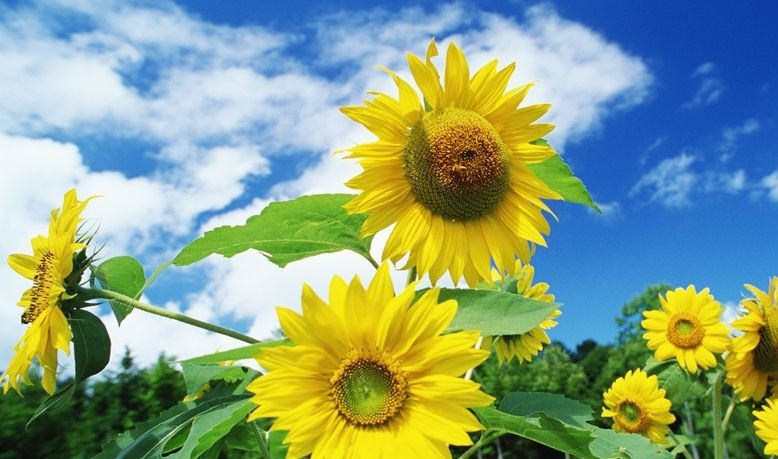
\includegraphics[width=1\textwidth]{./umetnine/soncnice.jpg}
  \caption{Tu bo neka slikica, ki bo lepa.}
  \label{fig:teaser}
\end{figure}
%

\section{Programerski del}
% TODO
% 4 STRANI SI LAHKO PRIVOŠČIMO